\documentclass[aspectratio=169]{beamer}
\usepackage[utf8]{inputenc}
\usepackage{tikz}
\usepackage{svg}
\usetheme[noto, showmaxslides]{pureminimalistic}
\usepackage{appendixnumberbeamer}
\usepackage[backend=biber, doi=false, maxbibnames=2, maxcitenames=2,style=numeric, sorting=none, url=false, eprint=false]{biblatex}
\addbibresource{references.bib}

\renewcommand{\appendixname}{\texorpdfstring{\translate{appendix}}{appendix}}
\renewcommand{\logotitle}{\includesvg[width=.2\linewidth]{logos/unibo-logo.svg}}
\renewcommand{\logoheader}{}
\renewcommand{\logofooter}{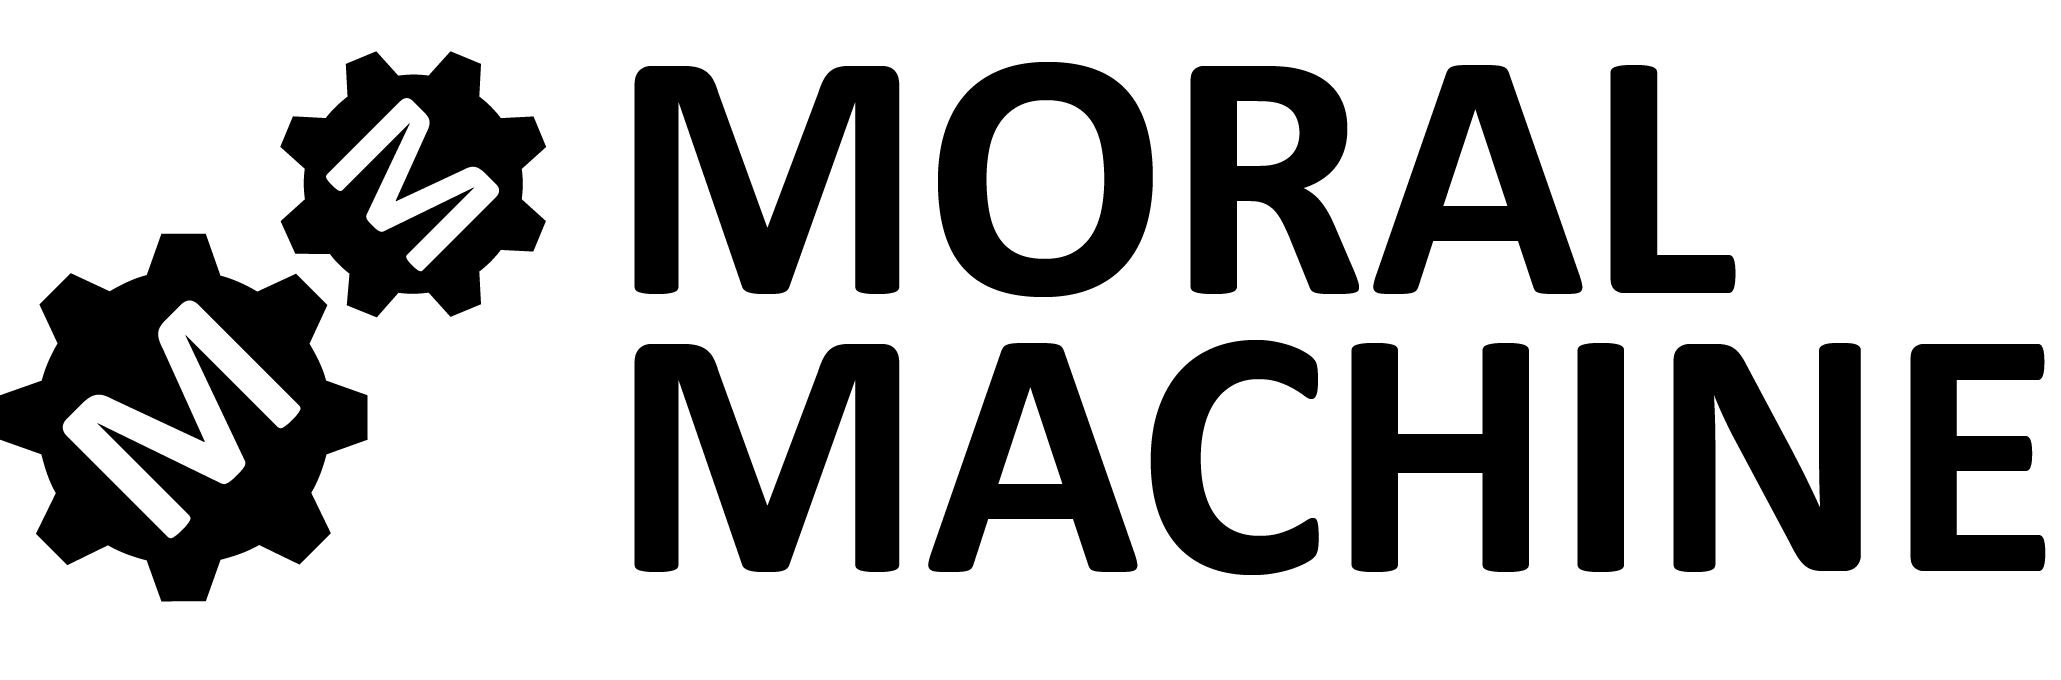
\includegraphics[width=.5\linewidth]{logos/mme-logo.png}}

\definecolor{bg}{RGB}{236, 240, 241}
\definecolor{text}{RGB}{52, 73, 94}
\definecolor{title}{RGB}{231, 76, 60}
\renewcommand{\beamerbgcolor}{bg}
\renewcommand{\beamertextcolor}{text}
\renewcommand{\beamertitlecolor}{title}

\title[MME]{The Moral Machine Experiment}
\author{Leonardo Calbi, Lorenzo Cellini, Alessio Falai\\}
\institute{Alma Mater Studiorum - University of Bologna}
\date{\today}

\begin{document}
\maketitle

% TOC
\begin{frame}[plain, noframenumbering]{Outline}
    \tableofcontents
\end{frame}

% Introduction
\section{Why ethics matters for autonomous cars}
\begin{frame}
    Introduction
\end{frame}

\section{The Moral Machine Experiment}

\begin{frame}
    \frametitle{Introduction}
    \begin{columns}[T]
        \begin{column}{0.5\linewidth}
        \begin{itemize}
            \item An online experimental platform designed to gauge social expectections about how autonomous vehicles should solve moral dilemmas.
            \item Almost 40M decisions from 233 different countries in 10 languages.
            \item Brakes failed what would you do?
            \begin{itemize}
                \item keep the lane and hit pedestrians on the road?
                \item swerve and hit pedestrians on the other lane?
                \item hit a barrier with the car?
            \end{itemize}
            \item What happens to the chosen characters?
            \begin{itemize}
                \item Skull \rightarrow Death
                \item Medical cross \rightarrow Injury
                \item Question mark \rightarrow Unknown
            \end{itemize}
        \end{itemize}
        \end{column}
        \begin{column}{0.5\linewidth}
            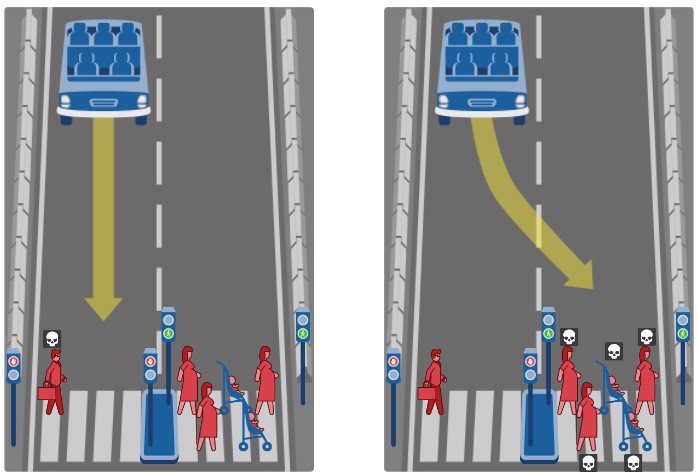
\includegraphics{assets/example-mme.jpg}
        \end{column}
    \end{columns}
\end{frame}

\begin{frame}
    \frametitle{Analysis framework}
    \begin{itemize}
        \item sparing humans (versus pets)
        \item staying on course (versus swerving)
        \item sparing passengers (versus pedestrians)
        \item sparing more lives (versus fewer lives)
        \item sparing men (versus women)
        \item sparing the young (versus the elderly)
        \item sparing pedestrians who cross legally (versus jaywalking)
        \item sparing the fit (versus the less fit)
        \item sparing those with higher social status (versus lower social status)
    \end{itemize}
\end{frame}

\begin{frame}
    \frametitle{Relative importance over the nine preferences}
    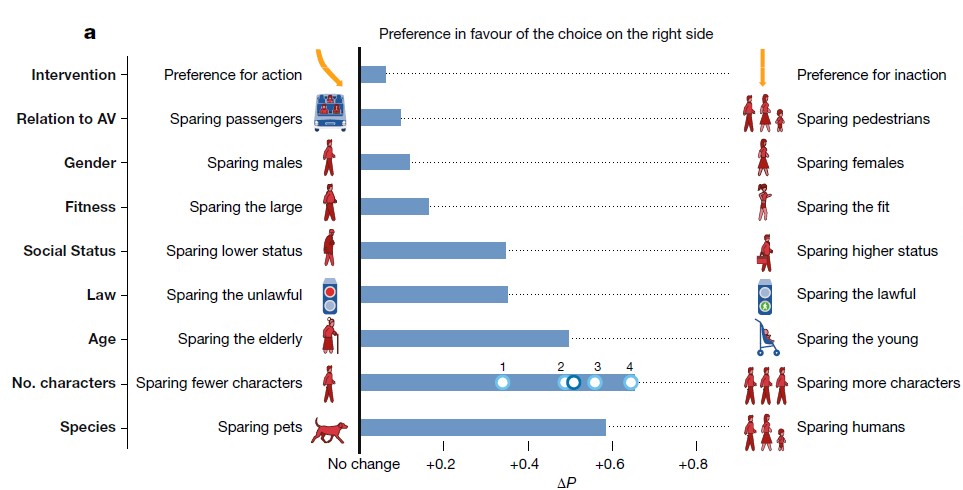
\includegraphics{assets/relative-importance-mme.jpg}
\end{frame}

\begin{frame}
    \frametitle{Hierarchical clustering of countries}
    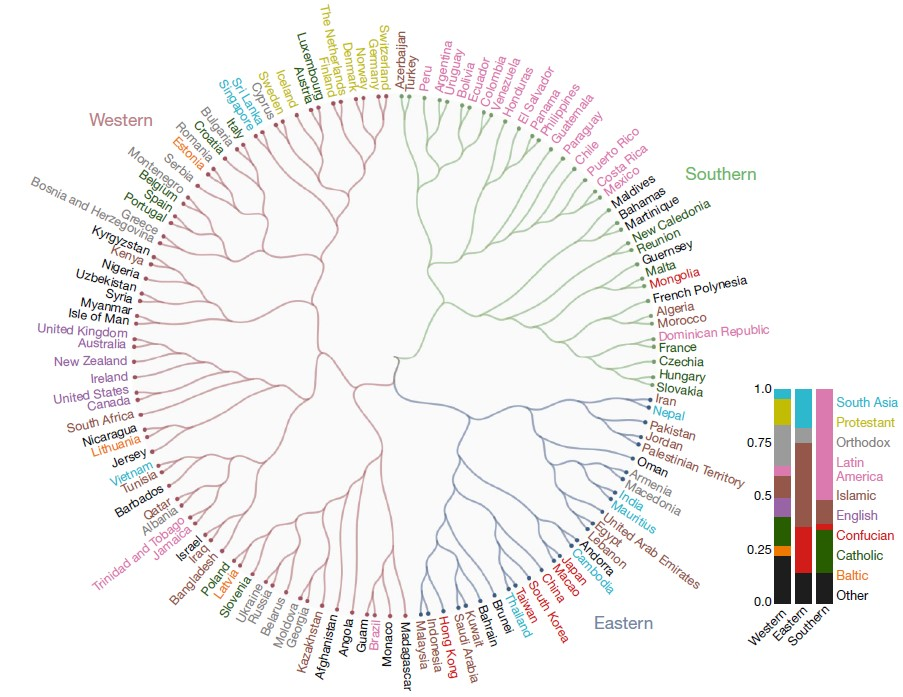
\includegraphics{assets/countries-mme.jpg}
\end{frame}

\begin{frame}
    \frametitle{Clusters preferences}
    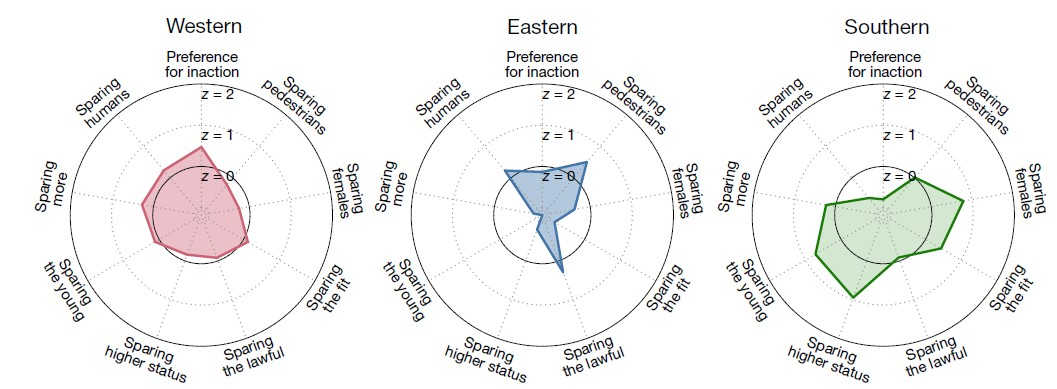
\includegraphics{assets/clusters-mme.jpg}
\end{frame}

\section{Arguments against MME}
\begin{frame}
    Life and Death decisions of autonomous
\end{frame}

\section{Conclusions}
\begin{frame}
    \cite{mme}
\end{frame}

\appendix
\begin{frame}[plain, noframenumbering]{References}
    \printbibliography
\end{frame}

\section*{Backup frames}
\begin{frame}[plain, noframenumbering]
    \centering
    \vfill
    {\fontsize{40}{50}\selectfont Backup frames}
    \vfill
\end{frame}

\begin{frame}{Backup demo}
    Demo
\end{frame}

\end{document}
